\documentclass[xcolor=dvipsnames, 14pt]{beamer}
\useoutertheme{infolines} 
\usecolortheme[named=OliveGreen]{structure} 
\usetheme[height=9mm]{Rochester}
\usepackage[utf8]{inputenc}
\usepackage{amsmath}
\usepackage{amsfonts}
\usepackage{amssymb}
\usepackage{graphicx}
\usepackage{epsfig}
\usepackage{caption}  
\usepackage{subcaption} 
\author[Lucio, Oakes, Vangheluwe]{Levi Lucio, Bentley James Oakes, and Hans Vangheluwe}
\title[Sym. Veri. of Translation Model Trans.]{Symbolic Verification of
Translation Model Transformations}

\AtBeginSection[]
{
   \begin{frame}
       \frametitle{Outline}
       \tableofcontents[currentsection]
   \end{frame}
}

%\setbeamercovered{transparent} 
\setbeamertemplate{navigation symbols}{} 
%\logo{} 
%\institute{} 
\date{\today} 
%\subject{} 
\begin{document}

\begin{frame}
\titlepage
\end{frame}

\begin{frame}
\tableofcontents
\end{frame}

\section{Overview}
\begin{frame}{Overview}
\begin{itemize}
\item Motivation is to formally prove properties on model transformations
\item A method to construct set of path conditions for a DSLTrans transformation
\item Set of path conditions represent all possible transformation executions
\item Prove structural properties on path conditions implies properties proved on transformation
\item Method is transformation-independent and graph-based
\end{itemize}
\end{frame}

\begin{frame}{Contributions}
\begin{itemize}
\item Algorithm to construct path conditions
\item Algorithm to prove properties on these path conditions
\item Validity and completeness proofs of these algorithms
\item Performance and scalability results
\end{itemize}
\end{frame}

\section{DSLTrans}
\begin{frame}{DSLTrans Overview}
\begin{itemize}


\item Transformation language
\item Turing-incomplete and outplace
\begin{itemize}
\item Avoids unbounded recursion or non-determinism
\item Allows construction of provably-finite set of path conditions
\end{itemize}
\item Transformation composed of rules in layers
\begin{itemize}
\item Rules in first layer are repeatedly executed in deterministic random order until exhausted
\item Next layer of rules is then executed
\end{itemize}
\end{itemize}
\end{frame}

\begin{frame}{Metamodels for Running Example}
\begin{figure}[htb]
        \centering
        \begin{subfigure}[b]{0.50\textwidth}
                \centering
                \includegraphics[width=1\textwidth]{../figures/policestation_dsltrans/squadagent.png}
                \caption{Chains of command}
                \label{fig:OrganizationLanguage}
        \end{subfigure}%
        ~~
        \begin{subfigure}[b]{0.50\textwidth}
                \centering
                \includegraphics[width=1\textwidth]{../figures/policestation_dsltrans/squadsex.png}
                \caption{Gender classification view}
                \label{fig:GenderLanguage}
        \end{subfigure}%
        %\caption{Metamodels for the Police Station Running Example}
        \label{fig:squadmetamodel}
\end{figure}
\end{frame}



\begin{frame}{Example DSLTrans Transformation}
\begin{figure}[h!]
	\centering
		\includegraphics[width=1\textwidth]{../figures/policestation_dsltrans/police_station_transformation.pdf}
	%\caption{A model transformation expressed in DSLTrans}
	\label{fig:dsltransformation}
\end{figure}
\end{frame}

\begin{frame}{Model Before/After Transformation}
Objective is to flatten a chain of command given in the Organization language language into two independent sets of male and female officers represented in the Gender language
\begin{figure}[htb]
        \centering
        \begin{subfigure}[b]{0.40\textwidth}
                \centering
                \includegraphics[width=1\textwidth]{../figures/policestation_dsltrans/model_police_hierarchy.pdf}
                \caption{Original model}
                \label{fig:police_hierarchy}
        \end{subfigure}%
        ~~
        \begin{subfigure}[b]{0.50\textwidth}
                \centering
                \includegraphics[width=1\textwidth]{../figures/policestation_dsltrans/model_police_gender.pdf}
                \caption{Transformed model}
                \label{fig:police_gender}
        \end{subfigure}%
        %\caption{Model before and after transformation}
        \label{fig:transformationexample}
\end{figure}
\end{frame}

\section{Path Condition Construction}

\begin{frame}{Path Conditions}
\begin{itemize}
\item Similar to symbolic path in symbolic execution
\item Formally represents concrete transformation executions
\item Composed of a match graph and an apply graph
\begin{itemize}
\item Path conditions look almost identical to DSLTrans rules
\end{itemize}
\end{itemize}
\end{frame}

\subsection{Building Path Constructions from Layers}

\begin{frame}{Rule Combinations}
\begin{itemize}
\item Take powerset of rules in first layer
\begin{itemize}
\item A, AB, ABC, BC
\item Abstract over number of times a rule executes
\end{itemize}
Also add traceability information to rules at this time
\end{itemize}

\end{frame}

\begin{frame}{Path Conditions}
\begin{itemize}
\item Take rule combination i.e. AC
\item Union match graphs together
\item Union apply graphs together
\end{itemize}

\end{frame}

\subsection{Disambiguating Path Conditions}

\begin{frame}{Disambiguating}

Match elements may refer to same element during transformation execution. Therefore, must disambiguate (recursively).
\begin{figure}[htb]
        \centering
        \begin{subfigure}[b]{0.40\textwidth}
                \centering
                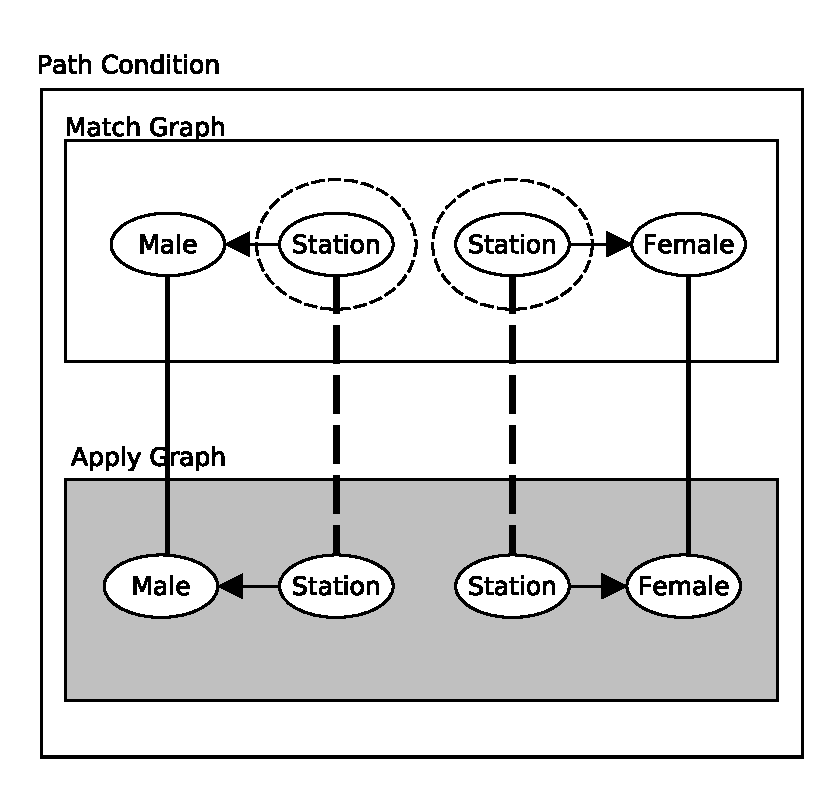
\includegraphics[width=1\textwidth]{../figures/building_path_conditions/collapse_locate_match.pdf}
                \caption{Locating elements}
                \label{fig:collapse_locate_match}
        \end{subfigure}%
        ~~
        \begin{subfigure}[b]{0.40\textwidth}
                \centering
                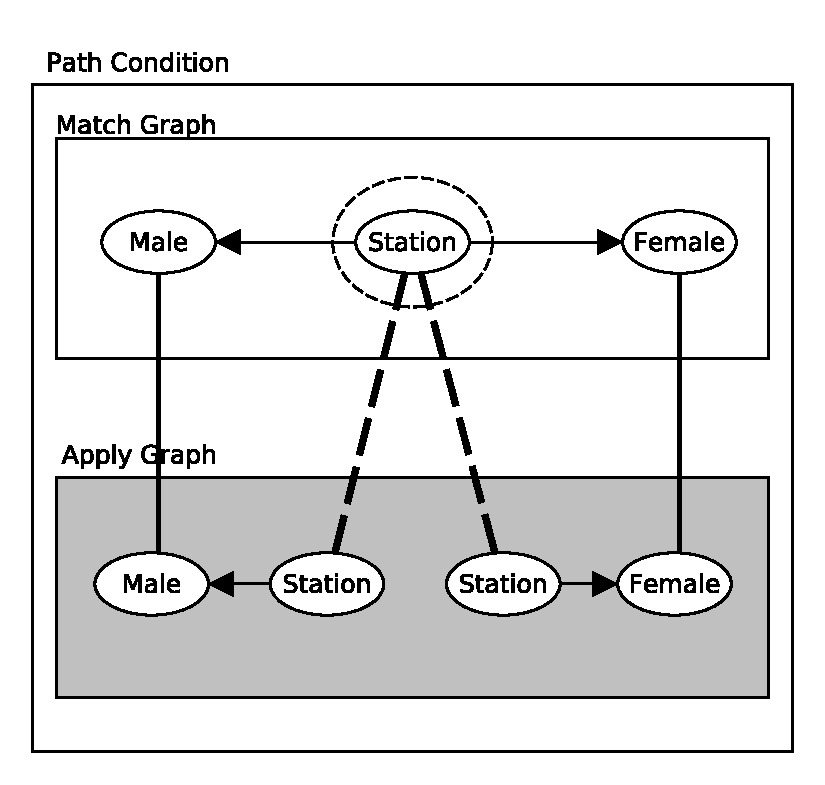
\includegraphics[width=1\textwidth]{../figures/building_path_conditions/collapse_merge_match.pdf}
                \caption{Merging elements}
                \label{fig:collapse_merge_match}
        \end{subfigure}%
        %\caption{Selecting and merging match elements of the same type}
        \label{fig:merge_match_elements}
\end{figure}
\end{frame}

\subsection{Generating All Path Conditions}

\begin{frame}{Combination Overview}
\begin{figure}[htb]
        \centering
        \begin{subfigure}[b]{0.55\textwidth}
                \centering
                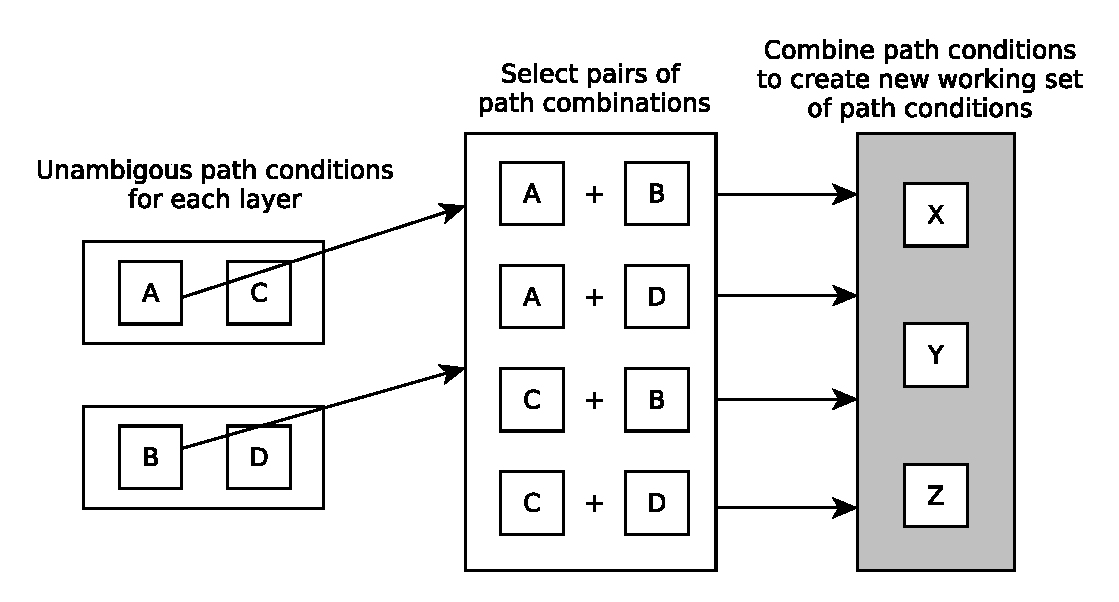
\includegraphics[width=1\textwidth]{../figures/building_path_conditions/combining_path_conditions.pdf}
                \caption{\textbf{Combining path conditions from two layers to produce working set of path conditions}}
                \label{fig:create_working_set}
        \end{subfigure}%
        ~
        \begin{subfigure}[b]{0.42\textwidth}
                \centering
                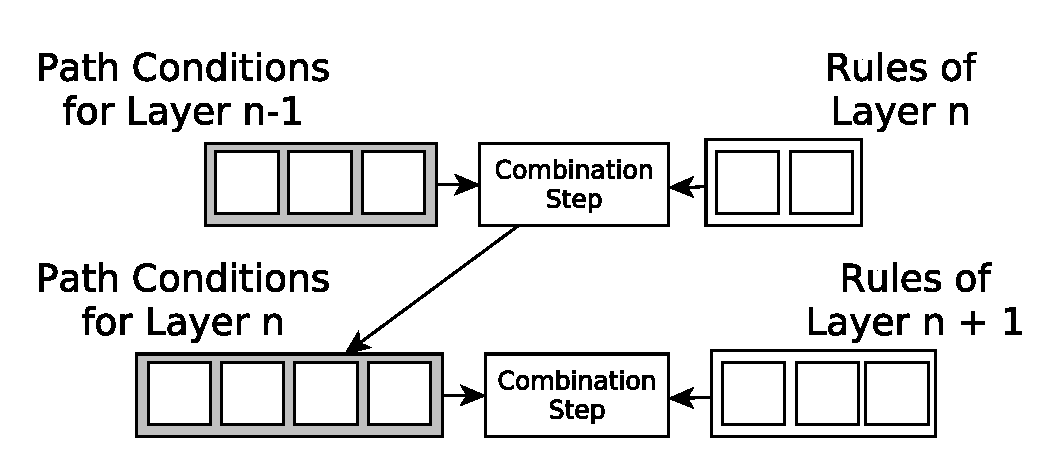
\includegraphics[width=1\textwidth]{../figures/building_path_conditions/next_layer.pdf}
                \caption{Combining the working set with the next layer's path conditions}
                \label{fig:combine_working_set}
        \end{subfigure}%
        %\caption{Combining path conditions from all layers}
        \label{fig:combining_path_conditions}
\end{figure}
\end{frame}

\begin{frame}{Combining Two Path Conditions}
\begin{itemize}
\item Take path conditions A from layer 1, and B from layer 2
\item Four different cases for combination
\begin{enumerate}
\item No interaction between A and B
\item A prevents B from holding
\item Both A and B \textit{may} hold
\item Both A and B \textit{will} hold
\end{enumerate}
\end{itemize}
Dependencies must be resolved by algorithm
\end{frame}

\begin{frame}{Path Condition Dependencies}
\begin{itemize}
\item Dependencies represented by backward link
\item Backward links are a construct in the DSLTrans rule language
\begin{itemize}
\item Enforce that a particular element in a apply graph was created from the connected element in the match graph
\end{itemize}
\end{itemize}
\begin{figure}[t]
                \centering
                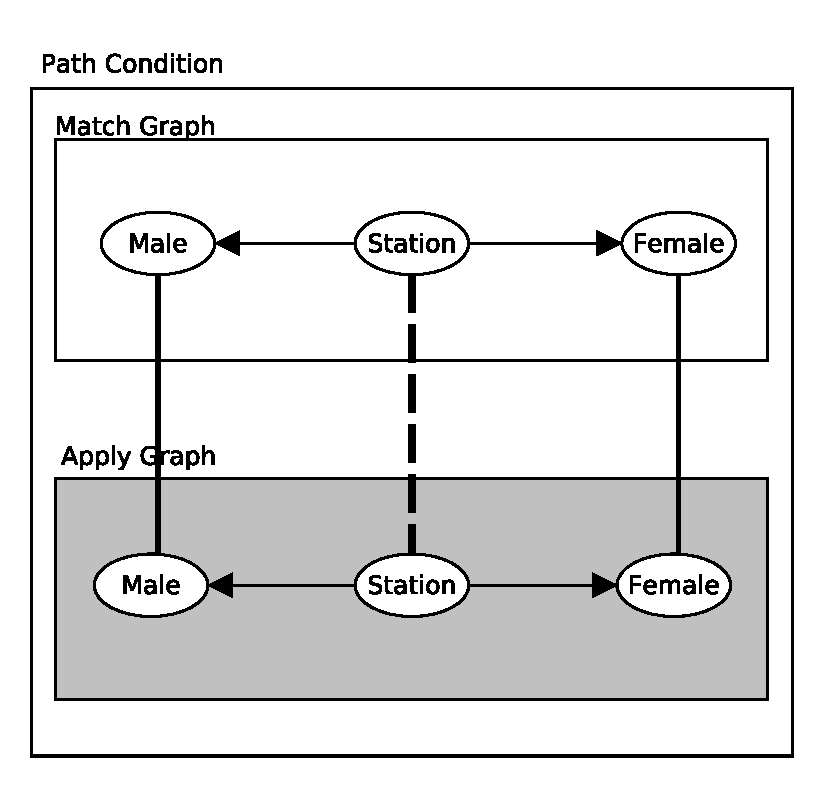
\includegraphics[height=0.66\textheight]{../figures/building_path_conditions/collapse_merge_apply.pdf}
                %\caption{Merging elements}
                \label{fig:collapse_merge_match}
\end{figure}
\end{frame}

\begin{frame}{Case 1}
\begin{figure}[h!] \centering 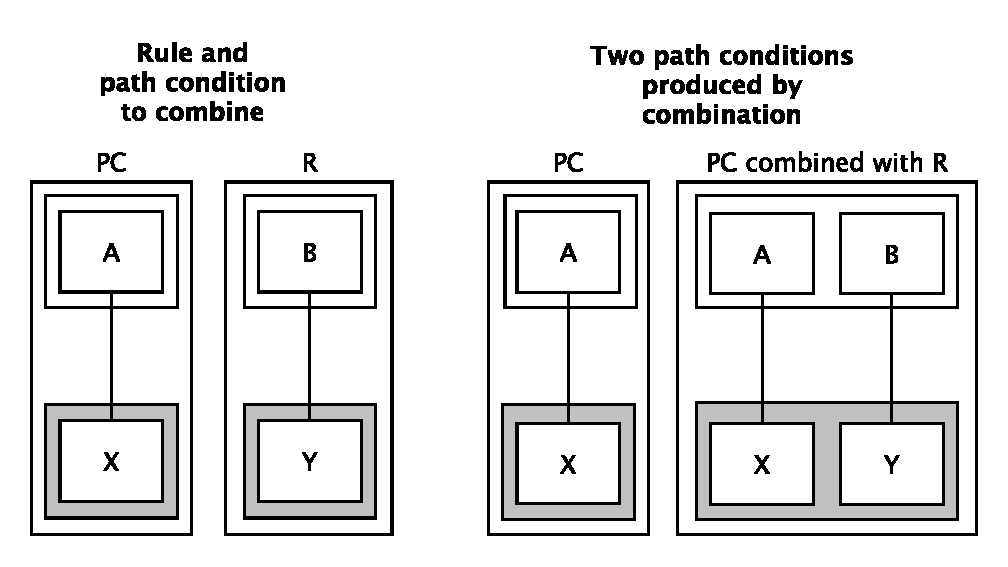
\includegraphics[width=0.7\textwidth]{../figures/building_path_conditions/no_dependencies.pdf}
	\caption{No dependencies between A and B}
	\label{fig:no_dependencies}
\end{figure}
\end{frame}

\begin{frame}{Case 2}
\begin{figure}[h!] \centering 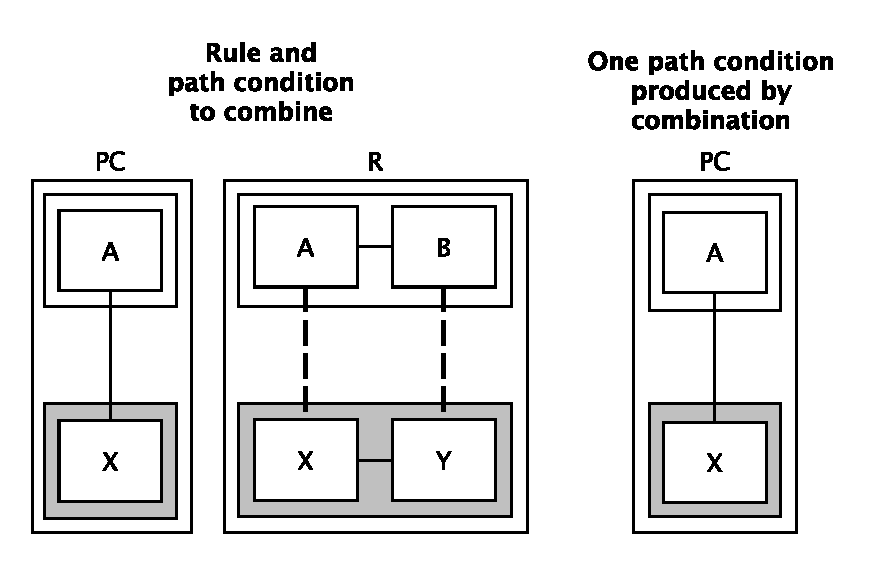
\includegraphics[width=0.7\textwidth]{../figures/building_path_conditions/non_satisfied_dependencies.pdf}
	\caption{B's dependencies are not satisfied by A}
	\label{fig:non_satisfied_dependencies}
\end{figure}
\end{frame}

\begin{frame}{Case 3}
\begin{figure}[h!] \centering 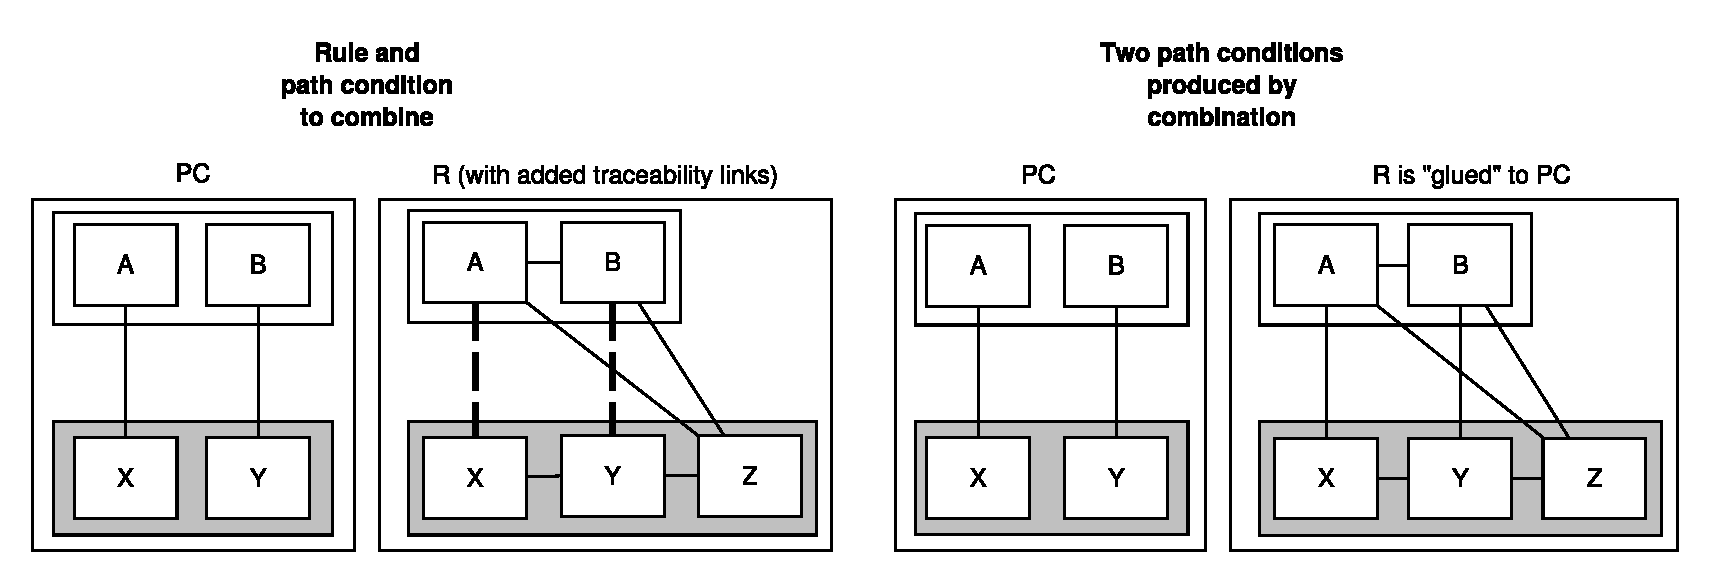
\includegraphics[width=\textwidth]{../figures/building_path_conditions/partial_satisfied_dependencies.pdf}
	\caption{B's dependencies are partially satisfied by A}
	\label{fig:partial_satisfied_dependencies}
\end{figure}
\end{frame}

\begin{frame}{Case 4}
\begin{figure}[h!] \centering 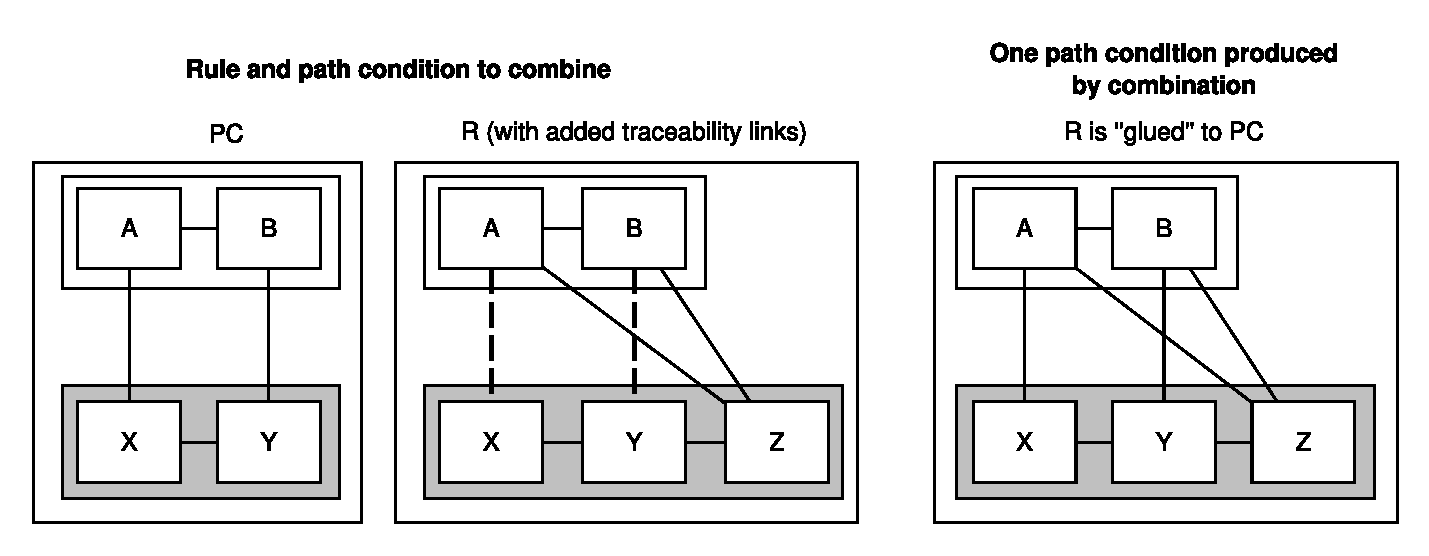
\includegraphics[width=\textwidth]{../figures/building_path_conditions/total_satisfied_dependencies.pdf}
	\caption{B's dependencies are fully satisfied by A}
	\label{fig:total_satisfied_dependencies}
\end{figure}
\end{frame}

\begin{frame}{Repeated Combinations}
\begin{figure}[htb]
        \centering
        \begin{subfigure}[b]{0.55\textwidth}
                \centering
                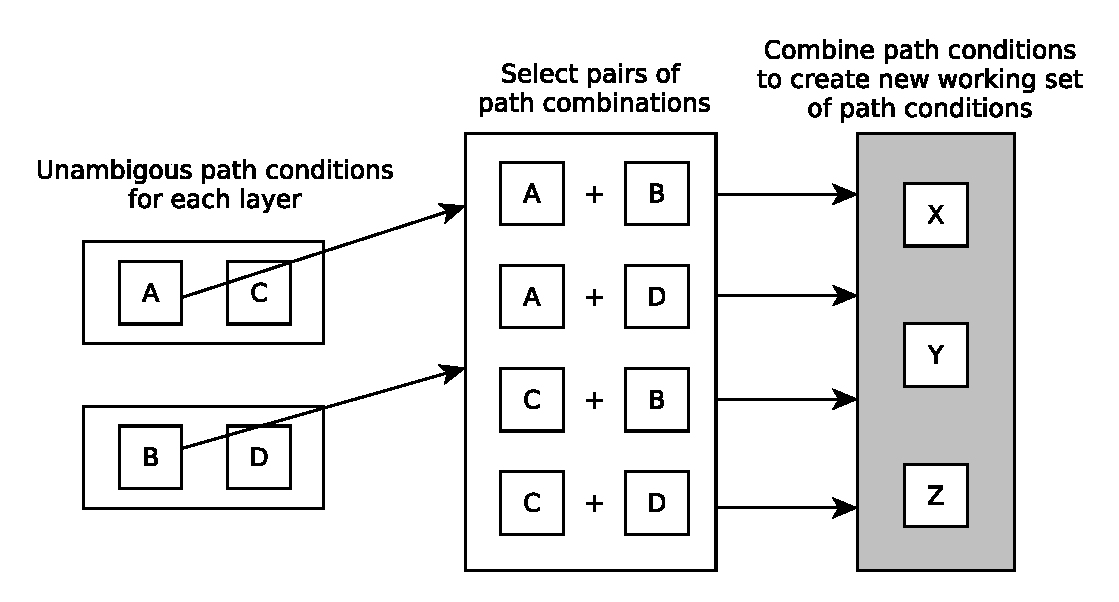
\includegraphics[width=1\textwidth]{../figures/building_path_conditions/combining_path_conditions.pdf}
                \caption{Combining path conditions from two layers to produce working set of path conditions}
                \label{fig:create_working_set}
        \end{subfigure}%
        ~
        \begin{subfigure}[b]{0.42\textwidth}
                \centering
                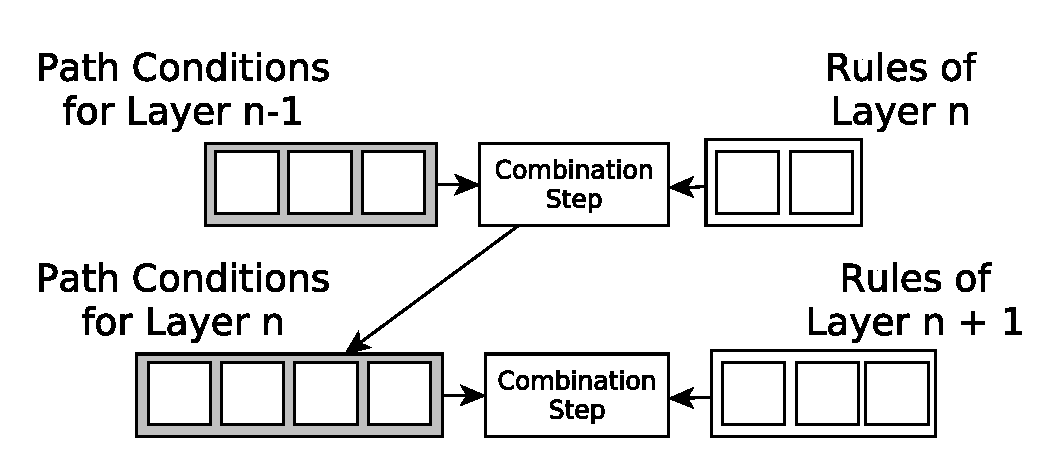
\includegraphics[width=1\textwidth]{../figures/building_path_conditions/next_layer.pdf}
                \caption{\textbf{Combining the working set with the next layer's path conditions}}
                \label{fig:combine_working_set}
        \end{subfigure}%
        %\caption{Combining path conditions from all layers}
        \label{fig:combining_path_conditions}
\end{figure}
\end{frame}

\section{Proving Properties}
\begin{frame}{Property Structure}
\begin{itemize}
\item Very similar to DSLTrans rules and path conditions
\item Composed of pre-condition and post-condition graphs
\end{itemize}

\end{frame}

\begin{frame}{Property Examples}
Property 1 -- Expected to hold: \small A model which includes a police station that has
both a male and female chief officers will be transformed into a model where the male
chief officer will exist in the male set and the female chief officer will exist in the female
set
\normalsize

\begin{figure}[htb]
        \centering
                \centering
                \includegraphics[height=.7\textheight]{../figures/policestation_dsltrans/satisfied.pdf}
                %\caption{Property 1 -- Expected to hold}
                \label{fig:dsltrans_prop1}

\end{figure}
\end{frame}
\begin{frame}{Property Examples}
Property 2 -- Not expected to hold: \small Any model which includes a female officer will
be transformed into a model where that female officer will always supervise another
female officer
\normalsize

\begin{figure}[htb]
        \centering
                \centering
                \includegraphics[height=.7\textheight]{../figures/policestation_dsltrans/unsatisfied.pdf}
                %\caption{Property 1 -- Expected to hold}
                \label{fig:dsltrans_prop1}

\end{figure}
\end{frame}

\begin{frame}{Repeated Combinations}
\begin{figure}[htb]
        \centering
        \begin{subfigure}[b]{0.55\textwidth}
                \centering
                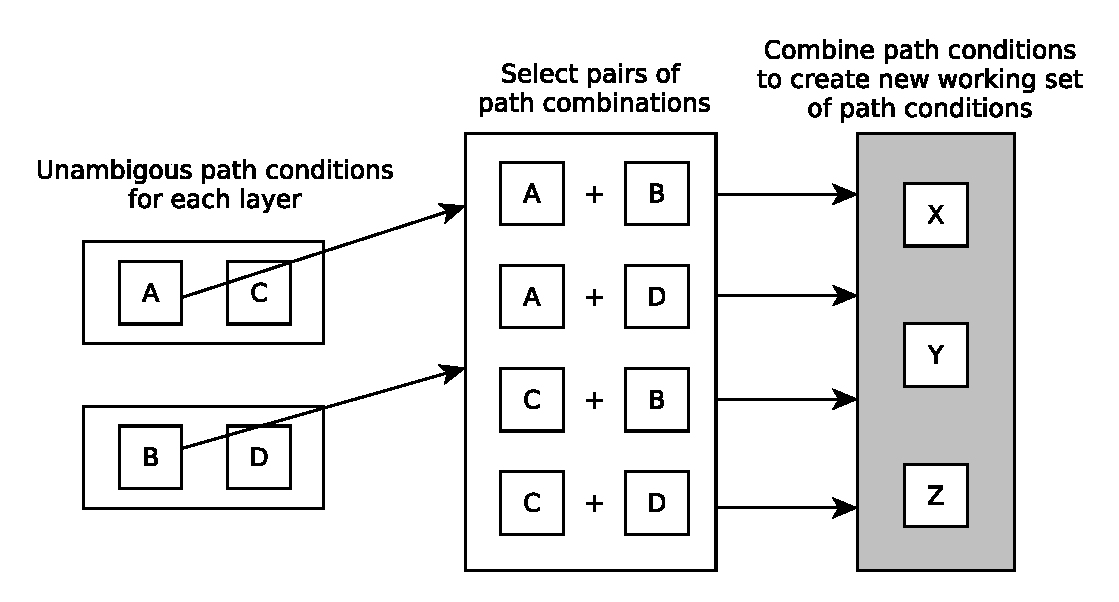
\includegraphics[width=1\textwidth]{../figures/building_path_conditions/combining_path_conditions.pdf}
                \caption{Combining path conditions from two layers to produce working set of path conditions}
                \label{fig:create_working_set}
        \end{subfigure}%
        ~
        \begin{subfigure}[b]{0.42\textwidth}
                \centering
                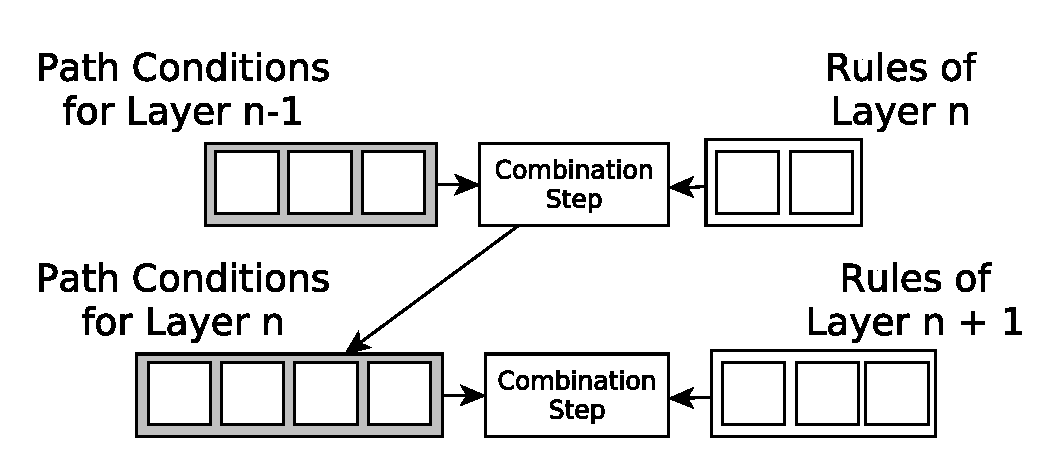
\includegraphics[width=1\textwidth]{../figures/building_path_conditions/next_layer.pdf}
                \caption{\textbf{Combining the working set with the next layer's path conditions}}
                \label{fig:combine_working_set}
        \end{subfigure}%
        %\caption{Combining path conditions from all layers}
        \label{fig:combining_path_conditions}
\end{figure}
\end{frame}

\section{Implementation}

\begin{frame}{Implementation Overview}
\begin{itemize}
\item Prototype built in Python and T-Core
\begin{itemize}
\item T-Core is library for efficiently matching/rewriting graphs
\end{itemize}
\item Naive complexity is calculated to be larger than O($2^{2*r}$) where $r$ is the number of rules in the transformation
\begin{itemize}
\item Complexity made worse when disambiguation is required
\end{itemize}
\item Optimizations such as memoisation/caching/lazy disambiguation performed
\end{itemize}
\end{frame}

\begin{frame}{Metrics for PC Creation}
\begin{figure}[htb]
        \centering
        \begin{subfigure}[b]{0.40\textwidth}
                \centering
                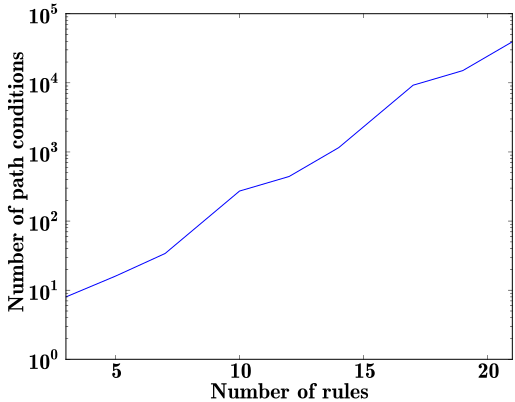
\includegraphics[width=1\textwidth]{../figures/results/rules_vs_pcs.pdf}
                \caption{Number of rules vs. path conds. created}
                \label{fig:rules_vs_pcs}
        \end{subfigure}%
        ~~
        \begin{subfigure}[b]{0.40\textwidth}
                \centering
                \includegraphics[width=1\textwidth]{../figures/results/rules_vs_time.pdf}
                \caption{Number of rules vs. time taken}
                \label{fig:rules_vs_time}
        \end{subfigure}%

        %\caption{Metrics for the path condition creation process}
        %\label{fig:path_condition_building}
\end{figure}
\footnotesize
\begin{tabular}{|p{1.3cm}|c|c|c|c|c|c|c|c|c|}
\hline
Rules & 3&  5&  7&  10&  12&  14 & 17 & 19 & 21\\\hline
Path conds. created & 8&  16&  34&  272&  442&  1156 & 9248 & 15028 & 39304\\\hline
Time taken(s) & 0.01&  0.13&  0.39&  1.87&  2.68&  9.00 & 59.08 & 97.52 & 369.19\\
\hline
\end{tabular}
\normalsize
\end{frame}

\begin{frame}{Metrics for PC Creation}
\begin{figure}[htb]
        \centering
        \begin{subfigure}[b]{0.5\textwidth}
                \centering
                \includegraphics[width=1\textwidth]{../figures/results/rules_vs_memory.pdf}
                \caption{Number of rules vs. memory used}
                \label{fig:rules_vs_pcs}
        \end{subfigure}%
        

        %\caption{Metrics for the path condition creation process}
        %\label{fig:path_condition_building}
\end{figure}
\footnotesize
\begin{tabular}{|p{1.6cm}|c|c|c|c|c|c|c|c|c|}
\hline
Rules & 3&  5&  7&  10&  12&  14 & 17 & 19 & 21\\\hline
Memory used (KB) & 0.08&  0.096&  0.17&  1.24&  1.83& 4.98 & 38.01 & 60.10 & 156.79\\
\hline
\end{tabular}
\normalsize
\end{frame}

\begin{frame}{Property-Proving Time}
\begin{figure}[htb]
        \centering
        \begin{subfigure}[b]{0.5\textwidth}
                \centering
                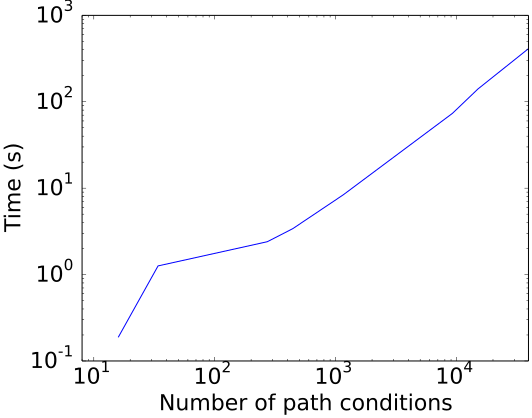
\includegraphics[width=1\textwidth]{../figures/results/pcs_vs_prop1.pdf}
                \caption{Time required to prove the property that holds on all path conditions}
                \label{fig:rules_vs_pcs}
        \end{subfigure}%
        

        %\caption{Metrics for the path condition creation process}
        %\label{fig:path_condition_building}
\end{figure}
\footnotesize
\begin{tabular}{|p{1.6cm}|c|c|c|c|c|c|c|c|c|}
\hline
Rules & 3&  5&  7&  10&  12&  14 & 17 & 19 & 21\\\hline
Proof time & -&  0.19&  1.26&  2.40&  3.40& 8.38 & 73.51 & 140.77 & 412.02\\
\hline
\end{tabular}
\normalsize
\end{frame}

\begin{frame}{Property-Proving Time}

For property that was not expected to hold for all path conditions, proof time is constant
\begin{itemize}
\item Algorithm detects counter-example quickly and does not need to process further path conditions
\end{itemize}

\normalsize
\end{frame}

\section{Concluding Material}
\begin{frame}{Contributions}

Contributions of this work include:
\begin{itemize}
\item Algorithm to construct a set of path conditions for a DSLTrans transformation
\item Property-checking algorithm to prove model syntax relation properties over these path conditions, and therefore over all concrete transformation executions
\item Validity and completeness proofs for the above algorithms (not shown in this presentation)
\item Discussion of optimisation and scalability concerns
\begin{itemize}
\item Successfully used in industrial case-study
\end{itemize}
\end{itemize}

\end{frame}


\begin{frame}{Future Work}

\begin{itemize}
\item Extend property language with attributes 
\item Negative DSLTrans constructs such as NACs
\item Application to further case studies
\item Develop tools to automatically create artifacts needed in algorithms
\begin{itemize}
\item Requires development of HOTs
\item Bentley is currently working on this, involves model evolution concerns
\end{itemize}
\end{itemize}

\end{frame}

\begin{frame}{Thank You}

This work has been developed in the context of the NECSIS project, funded by Automotive Partnership Canada.


\end{frame}

\end{document}